\documentclass[12pt]{article}
%\usepackage{xltxtra}
\usepackage{fancyhdr}
\usepackage{graphicx}
\usepackage{enumerate}
\usepackage{amsmath}
\usepackage{amssymb, bm}
\usepackage{subfigure}
\usepackage{hyperref}
\hypersetup{ %
	colorlinks=true,
    linkcolor=blue, %mydarkblue,
    citecolor=blue, %mydarkblue,
    filecolor=blue, %mydarkblue,
    urlcolor=blue, %mydarkblue,
} 
%\usepackage[utf8]{inputenc}
%\usepackage[T1]{fontenc}
%\usepackage{fontspec}
%\usepackage{xunicode}

\newcommand{\iid}{\stackrel{\text{iid}}{\sim}}
\newcommand{\eqInDist}{\stackrel{\text{d}}{=}}

\newcommand{\mysec}[1]{Section~\ref{sec:#1}}
\newcommand{\eq}[1]{Eq.~(\ref{eq:#1})}
\newcommand{\myfig}[1]{Figure~\ref{fig:#1}}

\newcommand{\BEAS}{\begin{eqnarray*}}
\newcommand{\EEAS}{\end{eqnarray*}}
\newcommand{\BEA}{\begin{eqnarray}}
\newcommand{\EEA}{\end{eqnarray}}
\newcommand{\BEQ}{\begin{equation}}
\newcommand{\EEQ}{\end{equation}}
\newcommand{\BIT}{\begin{itemize}}
\newcommand{\EIT}{\end{itemize}}
\newcommand{\BNUM}{\begin{enumerate}}
\newcommand{\ENUM}{\end{enumerate}}
\newcommand{\BA}{\begin{array}}
\newcommand{\EA}{\end{array}}
\newcommand{\diag}{\mathop{\rm diag}}
\newcommand{\var}{\mathop{\rm var}}
\newcommand{\mean}{\mathop{\rm mean}}
\newcommand{\Diag}{\mathop{\rm Diag}}

\newcommand{\nn}{\nonumber}
\newcommand{\half}{\frac{1}{2}}
\newcommand{\1}{{\bf 1}}
\newcommand{\st}{\text{ s.t.}}
\newcommand{\ie}{\text{ i.e.}}
\newcommand{\rb}{\mathbb{R}}
\newcommand{\cb}{\mathbb{C}}
\newcommand{\zb}{\mathbb{Z}}
\newcommand{\tr}{{\rm tr}}
\newcommand{\idm}{I}
\newcommand{\BlackBox}{\rule{1.5ex}{1.5ex}}  % end of proof
\newcommand{\indep}{\bot\!\!\!\bot}


\newenvironment{proof}{\par\noindent{\bf Proof\ }}{\hfill\BlackBox\\[2mm]}

\newtheorem{proposition}{Proposition}
\newtheorem{lemma}{Lemma}


% If your paper is accepted, change the options for the package
% aistats2e as follows:
%
%\usepackage[accepted]{aistats2e}
%
% This option will print headings for the title of your paper and
% headings for the authors names, plus a copyright note at the end of
% the first column of the first page.
\setlength{\parindent}{0cm}
%\ifMain
\addtolength{\oddsidemargin}{-2cm}
\addtolength{\evensidemargin}{-2cm}
\setlength{\textwidth}{17.78cm}
\addtolength{\topmargin}{-2.7cm}
\setlength{\textheight}{24.24cm}
%\else
\addtolength{\parskip}{5mm}
%\fi
\pagestyle{fancy}

\title{Hwk 3}
\author{Simon Lacoste-Julien}

\begin{document}
\fancyhead{}
\fancyfoot{}

\fancyhead[R]{
  \begin{tabular}[b]{l}
    Name: \hspace{3cm} \\
    Student id: \hspace{3cm} \\
  \end{tabular}
  %\vspace*{10\baselineskip}
}
\fancyhead[L]{
  \begin{tabular}[b]{l}
    IFT6269-A2018  \\
    Prof: Simon Lacoste-Julien \\
  \end{tabular}
  %\vspace*{10\baselineskip}
}
\fancyhead[C]{
  \begin{tabular}[b]{c}
    {\bf Hwk 3} \\
    Due date: Oct 30, 2018
  \end{tabular}
}

%\vspace{0.3cm}

As usual, please hand in on paper form your derivations and answers to the questions. You can use any programming language for your source code (submitted on Studium as per the website instructions). All the requested figures should be printed on paper with clear titles that indicate what the figures represent.


\begin{enumerate}

%--------------------
%    Question 1
%--------------------
\item {\bf DGM (5 points)}  \\
\begin{minipage}[b]{0.7\textwidth}
Consider the directed graphical model $G$ on the right. 
Write down the implied factorization for any joint distribution $p \in \mathcal{L}(G)$.
Is it true that $X \indep Y \mid T$ for any $p \in \mathcal{L}(G)$? Prove or disprove.
\end{minipage}
\begin{minipage}{0.3\textwidth}
\vspace{-10mm}
\hspace{0.6cm}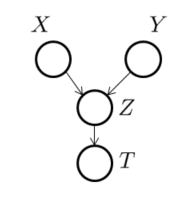
\includegraphics[scale=.5]{hwk3_GMex.png} \vspace{-10mm}
\end{minipage}

%--------------------
%    Question 2
%--------------------
\item {\bf d-separation in DGM (5 points)} \\
Indicate (yes or no) which conditional independence statements are true?

\hspace{0cm} 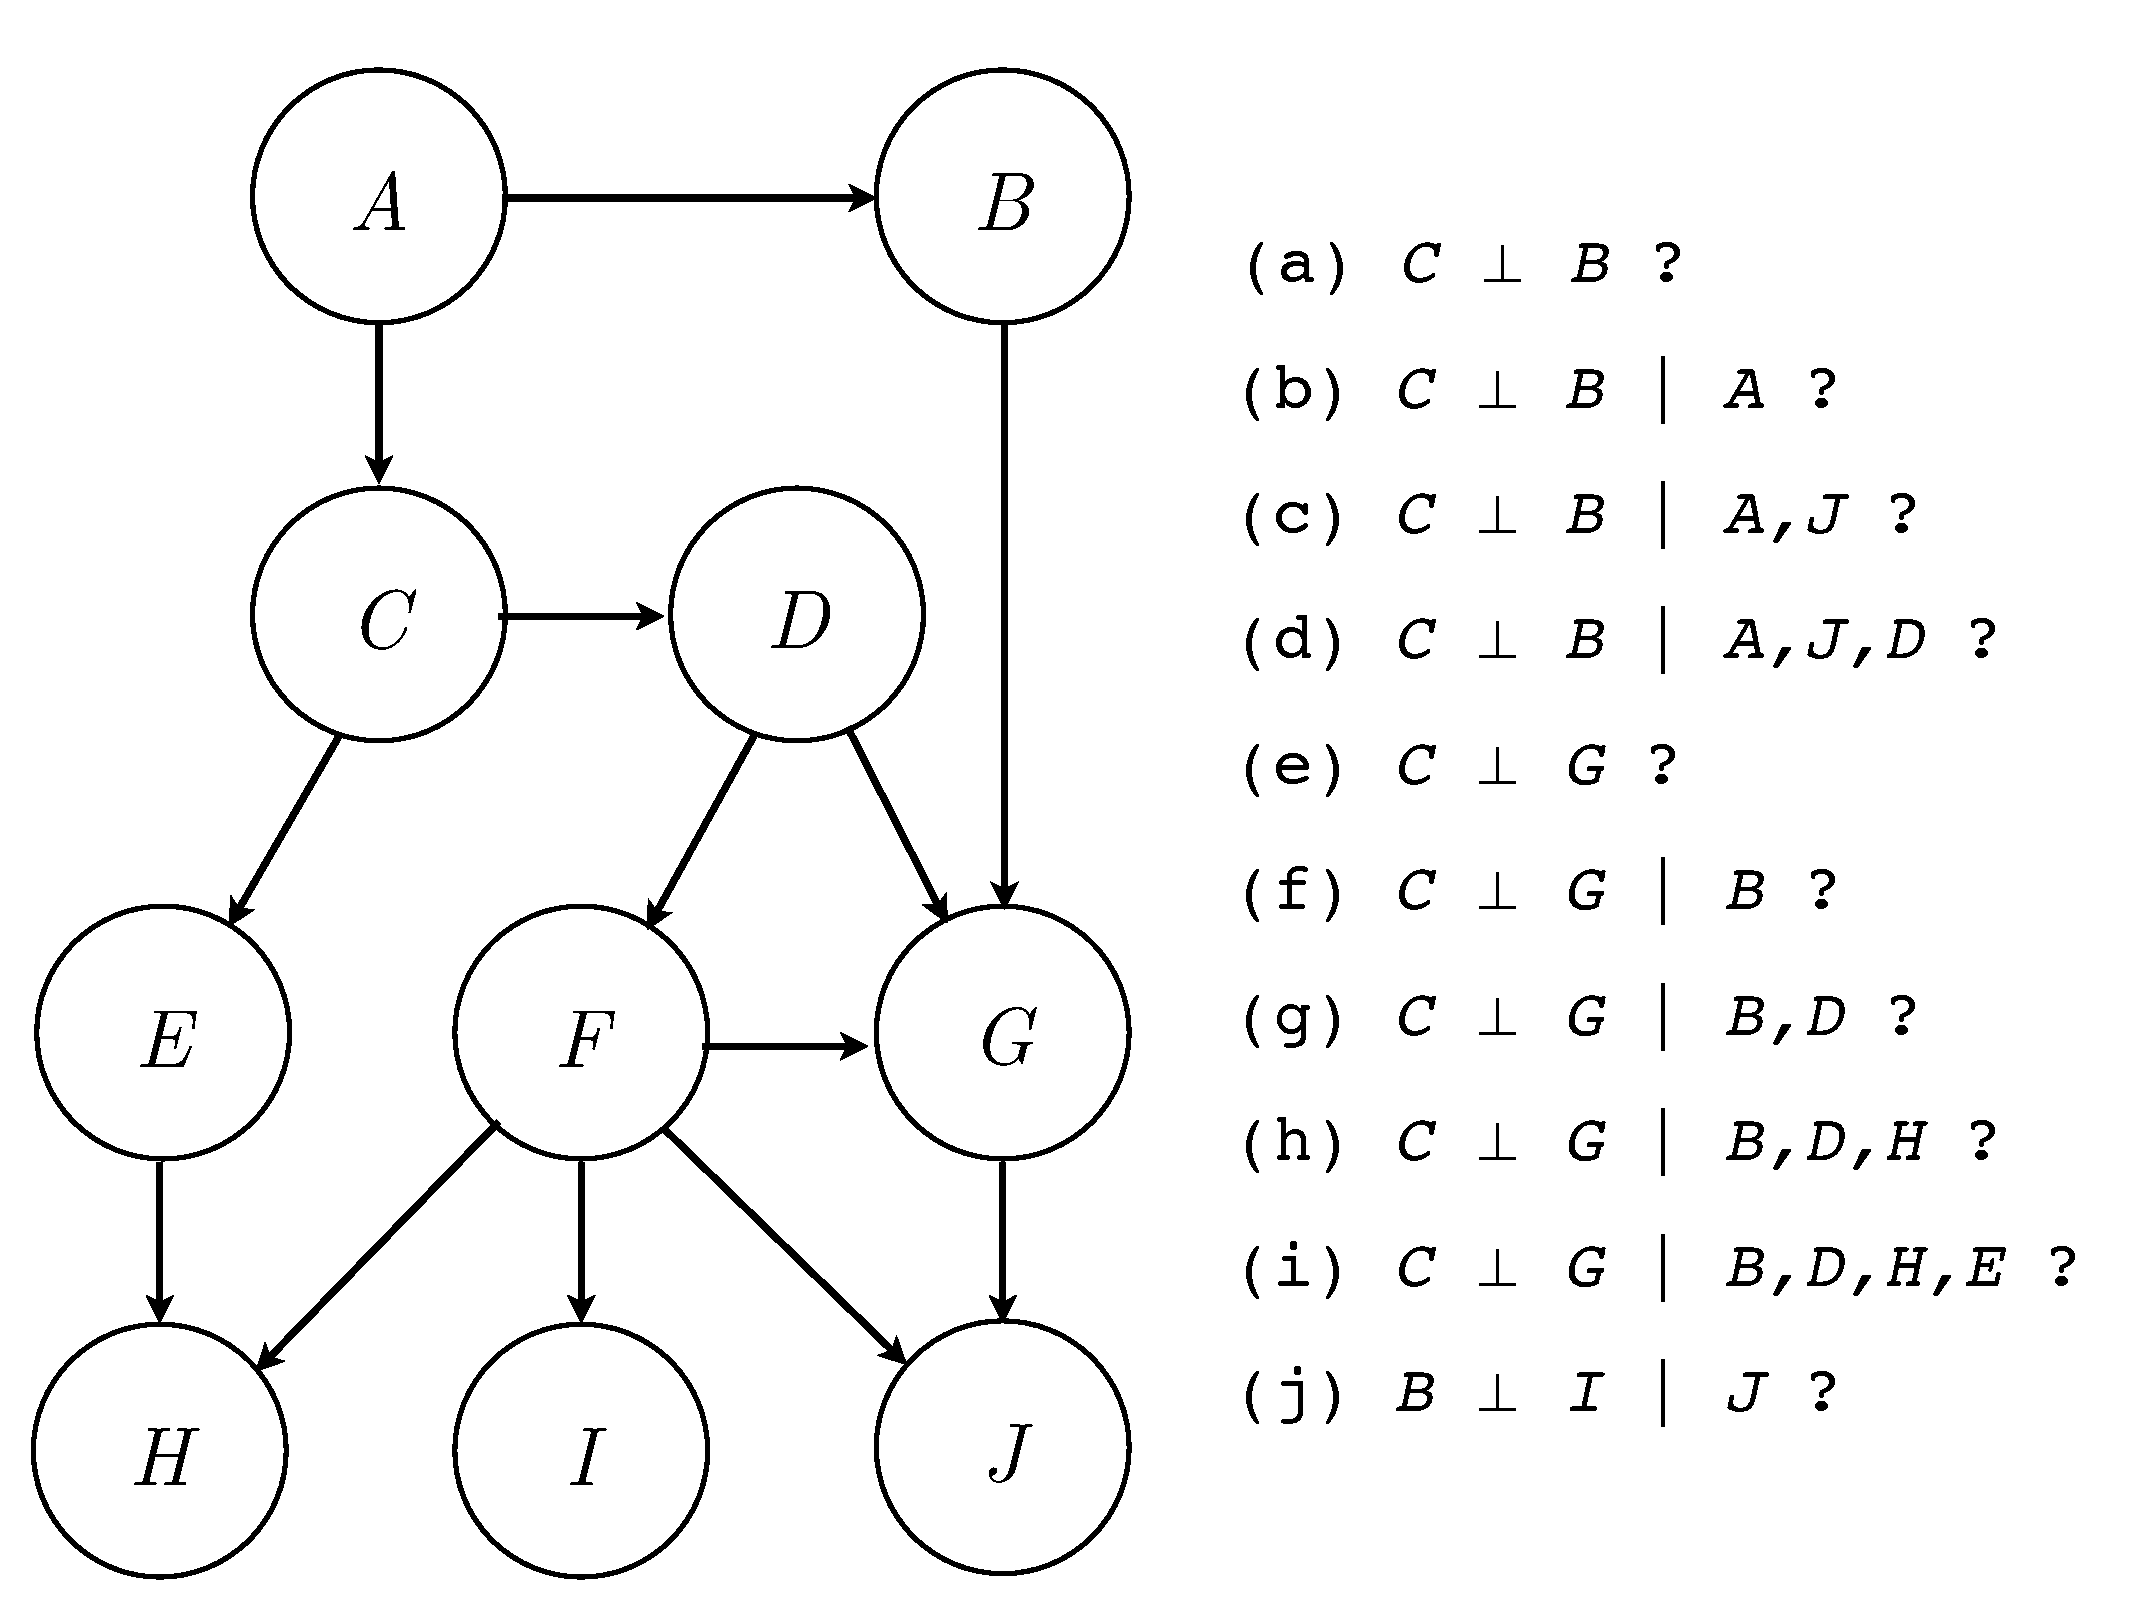
\includegraphics[scale=0.33]{hwk3_d-sep.pdf}

%--------------------
%    Question 3
%--------------------
% Get them to show the calculations for this question!!! 
% Assume p(x) = p(y) = 0.5
\vspace{5mm}
\item {\bf Positive interactions in-V-structure (10 points) } \\
Let $X, Y, Z$ be binary random variables with a joint
distribution parametrized according to the graph: $X \rightarrow Z
\leftarrow Y$. We define the following: 
\begin{equation}
a := P(X = 1), \quad b := P (X = 1 \mid Z = 1), \quad  c := P (X = 1 \mid Z
= 1, Y = 1) \nonumber
\end{equation}
\begin{enumerate}
\item For all the following cases, provide examples of conditional
probability tables (and calculate the quantities $a$, $b$, $c$),
that render the statements true: 
\begin{enumerate}[(i)]
\item $a> c$
\item $a <c <b$
\item $b <a <c$.
\end{enumerate}
\item Think of $X$ and $Y$ as causes and $Z$ as a common effect, for all
  the above cases (i, ii, et iii), summarize in a sentence or two why the
  declarations are true for your examples.
\end{enumerate}

%--------------------
%    Question
%--------------------
\item {\bf Flipping a covered edge in a DGM (10 points) } \\
Let $G=(V,E)$ be a DAG. We say that a directed edge $(i,j) \in E$ is a \emph{covered edge} if and only if $\pi_j=\pi_i \cup \{i\}$.
let $G'=(V,E')$, with $E'= ( E\backslash \{ (i,j)\} )\cup \{ (j,i)\}$. Prove that $\mathcal{L}(G)=\mathcal{L}(G')$.

\vspace{0.2cm}

%--------------------
%    Question
%--------------------
\item {\bf Equivalence of directed tree DGM with undirected tree UGM (10 points) } \\
Let $G$ be a directed tree and $G'$ its corresponding undirected tree (where the orientation of edges is ignored). Recall that by the definition of a directed tree, $G$ does not contain any v-structure. Prove that $\mathcal{L}(G)=\mathcal{L}(G')$.

\vspace{0.2cm}

%--------------------
%    Question
%--------------------
\item {\bf Hammersley-Clifford Counter example (10 points)} \\
In class, I mentioned that the strict positivity of the joint distribution was crucial in the Hammersley-Clifford theorem. Here is a counter-example that shows the problems when we have zero probabilities (it is example 4.4 in Koller \& Friedman). Consider a joint distribution~$p$ over four binary random
variables: $X_1$, $X_2$, $X_3$ and $X_4$ which gives probability
$\frac{1}{8}$ to each of the following eight configurations, and
probability zero to all others:
\[
\begin{array}{cccc}
(0,0,0,0) & (1,0,0,0) & (1,1,0,0) & (1,1,1,0) \\
(0,0,0,1) & (0,0,1,1) & (0,1,1,1) & (1,1,1,1) .
\end{array}
\]
Let $G$ be the usual four nodes undirected graph
$X_{1}\text{---}X_{2}\text{---}X_{3}\text{---}X_{4}\text{---}X_{1}$. One can show that $p$ satisfies the 
global Markov property with respect to this graph $G$ because of trivial deterministic relationships. For example, if we condition on $X_2 = 0$ and $X_4=0$, then the only value of $X_3$ with non-zero probability is $X_3 = 0$, and thus $X_3 | X_2=0 ,X_4=0$ being a deterministic random variable, it is trivially conditionally independent to $X_1$. By (painfully) going through all other possibilities, we get similar situations (for example $X_2=0$ and $X_4=1$ forces $X_1 = 0$, etc.). Prove that the
distribution $p$ \emph{cannot} factorize according to $G$ (and thus $p \notin \mathcal{L}(G)$). \emph{Hint: argue by contradiction.}

\vspace{0.2cm}

%--------------------
%    Question
%--------------------
\item {\bf [BONUS]: bizarre conditional independence properties (10 bonus points)} \\ 
Let $(X,Y,Z)$ be a random vector with a finite sample space. Consider the following statement: 
\begin{center}
``If  $X \indep Y \mid Z$ and $X \indep Y$ then ($X \indep Z$ or $Y \indep Z$).''
\end{center}
\BNUM
\item Is this true if one assumes that $Z$ is a binary variable? Prove or disprove.
\item Is the statement true in general? Prove or disprove.
\ENUM 


%--------------------
%    Question
%--------------------
\vspace{0.2cm}

\item {\bf Implementation: EM and Gaussian mixtures (30 points)} \\
The file \texttt{EMGaussian.train} contains samples of data  $x_i$ where $x_i \in \rb^2$ (one datapoint per row). The goal of this exercise is to implement the EM algorithm for some mixtures of $K$ Gaussians in $\rb^d$ (here $d=2$ and $K=4$), for i.i.d.~data.
(NB: in this exercise, no need to prove any of the formula used in the algorithms except for question (b)).

\BNUM
\item[(a)]
Implement the K-means algorithm. Represent graphically the training data, the cluster centers, as well as the different clusters (use 4 colors). Try several random initializations and compare results (centers and the actual K-means objective values).

\item[(b)]
Consider a Gaussian mixture model in which the covariance matrices are proportional to the identity.
Derive the form of the M-step updates for this model and implement the corresponding EM algorithm (using an initialization with K-means).

Represent graphically the training data, the centers, as well as the covariance matrices (an elegant way is to represent the ellipse that contains a specific percentage, e.g., 90\%, of the mass of the Gaussian distribution).

Estimate and represent (e.g. with different colors or different symbols) the most likely latent variables for all data points (with the parameters learned by EM).

\item[(c)]

Implement the EM algorithm for a Gaussian mixture with general covariance matrices. 
Represent graphically the training data, the centers, as well as the covariance matrices.

Estimate and represent (e.g. with different colors or different symbols) the most likely latent variables for all data points (with the parameters learned by EM).
 

\item[(d)] Comment the different results obtained in earlier questions. In particular, compare the normalized log-likelihoods of the two mixture models on the training data, as well as on test data (in \texttt{EMGaussian.test}). (Here normalize the log-likelihood by the number of observations (rows) -- it makes the number more manageable for comparison and puts it on the right scale).


\ENUM

\end{enumerate}

\end{document}


